
\chapter{Software Structure and Verification}

The mathematical and numerical robustness of a deterministic computer model depends upon
three issues: the code must be transparent so that it can be understood and modified by visual
inspection; it must be possible to check and verify the coding implementation (perhaps with automated tools); and there must be a
method for checking the correctness of the solution, at least for asymptotic (steady state)
solutions (numerical stability and agreement with known solutions).

The terms {\em verification} and {\em validation} are often used interchangeably to mean the process of checking the
accuracy of a numerical model. For many, this entails comparing model predictions with experimental measurements. However,
there is now a fairly broad-based consensus that comparing model and experiment is largely what is considered {\em validation}. So what is
{\em verification}? ASTM~E~1355~\cite{ASTM:E1355}, ``Standard Guide for
Evaluating the Predictive Capability of Deterministic Fire Models,'' defines verification as
\begin{quote}
The process of determining that the implementation of a calculation method accurately
represents the developer's conceptual description of the calculation method and the solution to the calculation method.
\end{quote}
and it defines validation as
\begin{quote}
The process of determining the degree to which a calculation method is an accurate representation of the real world
from the perspective of the intended uses of the calculation method.
\end{quote}
Simply put, verification is a check of the math; validation is a check of the physics. If the model predictions closely match
the results of experiments, using whatever metric is appropriate, it is assumed by most that the model suitably describes, via
its mathematical equations, what is happening. It is also assumed that the solution of these equations must be correct. So why do
we need to perform model verification? Why not just skip to validation and be done with it? The reason is that rarely do model and
measurement agree so well in all applications that anyone would just accept its results unquestionably. Because there is
inevitably differences between model and experiment, we need to know if these differences are due to limitations or errors in
the numerical solution, or the physical sub-models, or both.

Whereas model validation consists mainly of comparing predictions with measurements, as documented later in this guide, 
model verification consists of a much broader range of activities, from checking the computer program
itself to comparing calculations to analytical (exact) solutions to understanding the impact on model outputs from a range of different model inputs.

In order to understand the meaning model verification, it is also  necessary to understand the
means by which the numerical routines are structured. In this chapter, details of the
implementation of the model are presented, including the tests used to assess the numerical
aspects of the model. These include:

\begin{itemize}
\item the structure of the model, including the major routines implementing the various
physical phenomena included in the model,
\item the organization of data initialization and data input used by the model,
\item the structure of data used to formulate the differential equations solved by the model,
\item a summary of the main control routines in the model that are used to control all input and
output, initialize the model and solve the appropriate differential equation set for the
problem to be solved,
\item the means by which the computer code is checked for consistency and correctness,
\item analysis of the numerical implementation for stability and error propagation, and
\item comparison of the results of the system model with simple analytical or numerical
solutions.
\item a series of reference test cases used to evaluate the impact of model changes to the full range of model outputs.
\end{itemize}

\section{Structure of the Numerical Routines}

A methodology which is critical to verification of the model is the schema used to incorporate
physical phenomena. This is the subroutine structure discussed below. The method for
incorporating new phenomena and ensuring the correctness of the code was adopted as part of
the consolidation of CCFM and FAST. This consolidation occurred in 1990 and has resulted in a
more transparent, transportable and verifiable numerical model. This transparency is crucial to a
verifiable and robust numerical implementation of the predictive model as discussed in the
sections on code checking and numerical analysis.

The model can be split into distinct parts. There are routines for reading data, calculating results
and reporting the results to a file or printer. The major routines for performing these functions
are identified in figure \ref{figCFASTStructure}. These physical interface routines link the CFAST model to the actual routines which calculate quantities such as mass or energy flow at one particular point in time for a given environment.

\begin{figure}[\figoptions{b}]
\begin{center}
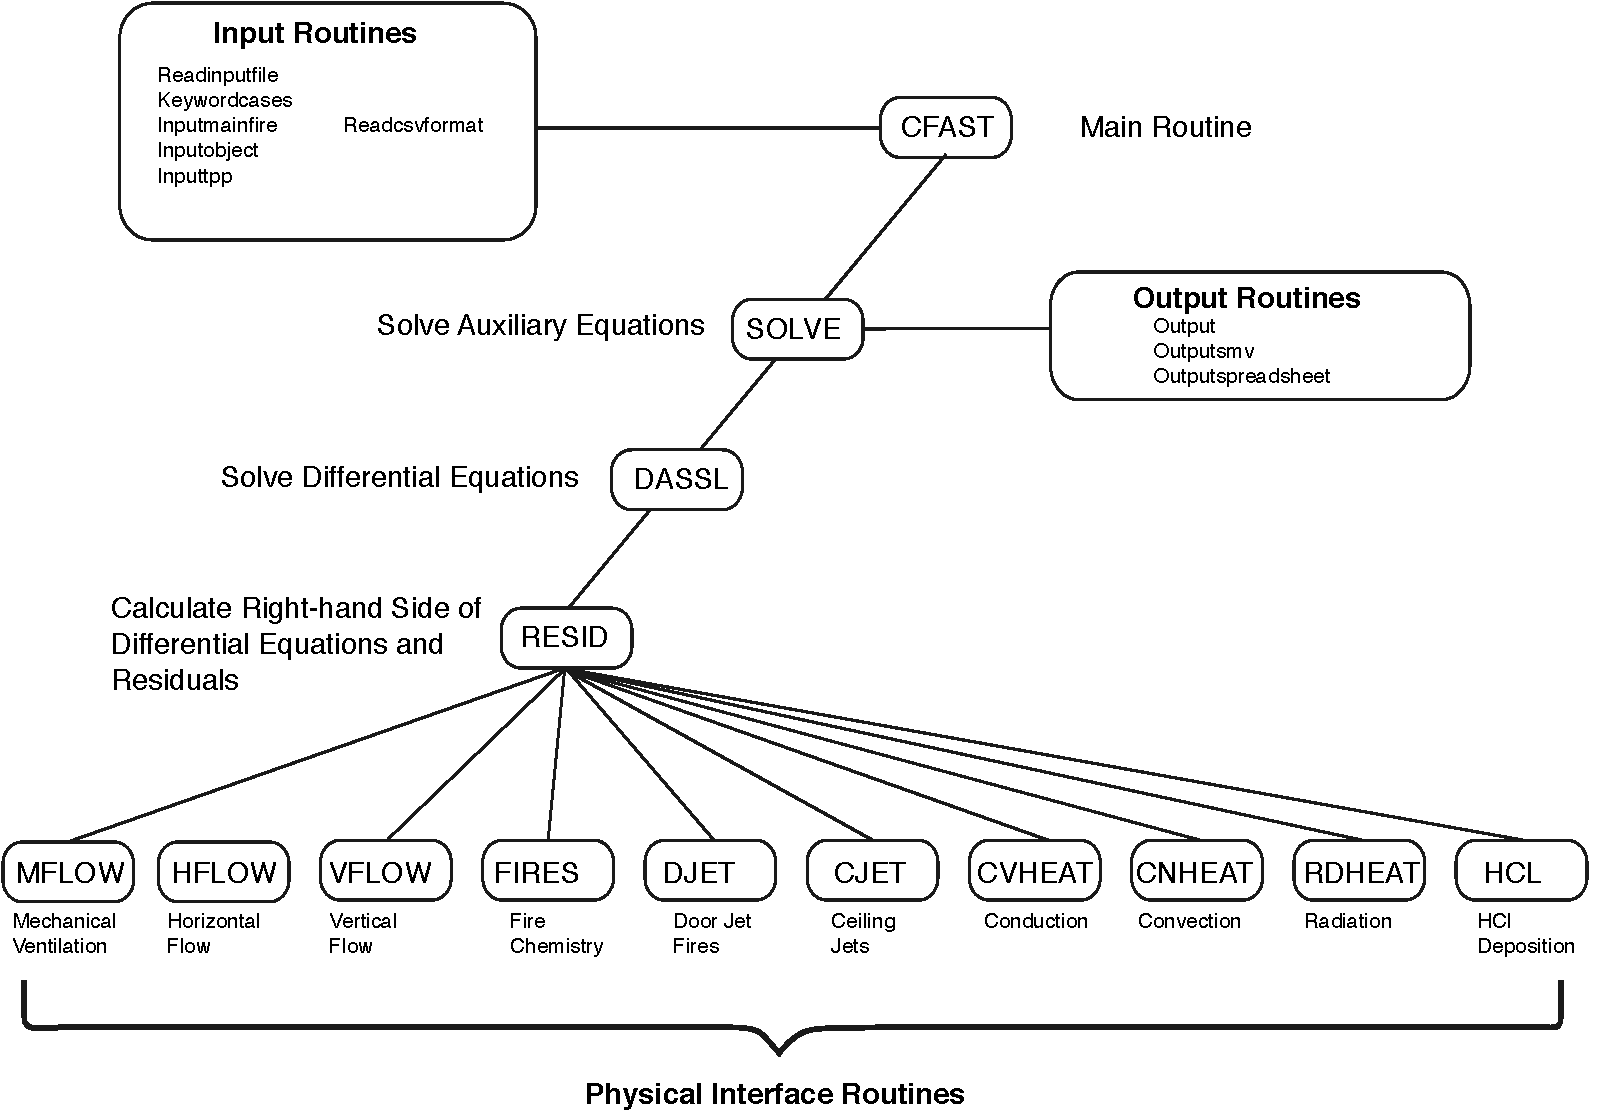
\includegraphics[width=4.4444in]{FIGURES/Structure}\\
\end{center}
\caption[Subroutine structure for the CFAST model]{Subroutine structure for the CFAST model showing major routines and calling structure.}
 \label{figCFASTStructure}
\end{figure}

The routines SOLVE, RESID and DASSL are the key to understanding how the physical
equations are solved. SOLVE is the control program that oversees the general solution of the
problem. It invokes the differential equation solver DASSL \cite{DASSL} which in turn calls RESID to
solve the transport equations. Given a solution at time t, what is the solution at time t plus a
small increment of time, $\dt$? The differential equations are of the form

\begin{eqnarray}
   \frac{{dy}}{{dx}} &=& f(y,t) \label{eqdiffeqform}  \\
    y(t_0 ) &=& y_0 \nonumber
\end{eqnarray}

where $y$ is a vector representing pressure, layer height, mass and such, and $f$ is a vector function that represents changes in these values with respect to time. The term $y_0$ is an initial condition at
the initial time $t_0$. The time increment is determined dynamically by the program to ensure convergence of the solution at $t + \Delta t$. The subroutine RESID computes the right hand side of eq \ref{eqdiffeqform} and returns a set of residuals of that calculation to be compared to the values expected by DASSL. DASSL then checks for convergence. Once DASSL reaches an error limit (defined as convergence of the equations) for the solution at $t + \Delta t$, SOLVE then advances the solution of species concentration, wall temperature profiles, and mechanical ventilation for the same time interval.
Note that there are several distinct time scales that are involved in the solution of this type of
problem. The fastest will be chemical kinetics. In CFAST, chemical reactions are assume to be instantaneous so we ignore the impact of chemical kinetics.  The next larger time scale is that associated with the flow field. These are the equations which are cast into the form of ordinary differential equations. Then there is the time scale for mechanical ventilation, and finally, heat conduction through objects.

Chemical kinetic times are typically on the order of milliseconds. The transport time scale are
on the order of 0.1 s. The mechanical ventilation and conduction time scales are typically
several seconds, or even longer. The time step is dynamically adjusted to a value appropriate for
the solution of the currently defined equation set. In addition to allowing a more correct solution
to the pressure equation, very large time steps are possible if the problem being solved
approaches steady-state.

\section{Numerical Tests}

CFAST is designed to use 64-bit precision for real number calculations to minimize the effects of numerical error.

The differential and algebraic equation solver (called DASSL) has been tested for a variety of differential equations and is widely used and accepted \cite{DASSL}.  The radiation and conduction routines have also been tested against known solutions for asymptotic results \cite{Forney_radiation}.

Coupling between the physical algorithms of the model and the differential equation solver also works to ensure numerical accuracy by dynamically adjusting the time step used by the model to advance the solutions of the equation set. Solution tolerances are set to require solution of the model equations within one part in $10{^6}$. This ensures that the error attributable to numerical solution is far less than that associated with the model assumptions.

\section{Code Checking}
Two standard programs have been used to check the CFAST model structure and language.  Specifically, FLINT and LINT have been applied to the entire model to verify the correctness of the interface, undefined or incorrectly defined (or used) variables and constants, and completeness of loops and threads.

The CFAST code has also been checked by compiling and running the model on a variety of computer platforms.  Because FORTRAN and C are implemented differently for various computers, this represents both a numerical check as well as a syntactic check.  CFAST has been compiled for Sun (Solaris), SGI (Irix), Microsoft Windows-based PCs (Lahey, Digital, and Intel FORTRAN), and Concurrent computer platforms.  Within the precision afforded by the various hardware implementations, the model outputs are identical on the different platforms. \footnote{Typically an error limit of one part in $10^6$ which is the limit set for the differential equation solver in the solution of the CFAST equations}

The CFAST Technical Reference Guide \cite{CFAST_Tech_Guide_6} contains a detailed description of the CFAST subroutine structure and interactions between the subroutines.

\section{Comparison with Analytical Solutions}

Certain CFAST sub-models address phenomena that have analytical solutions, for example, one dimensional heat conduction through a solid or pressure increase in a sealed or slightly leaky compartment as a result of a fire or fan.  The developers of CFAST use analytical solutions to test sub-models to verify the correctness of the coding of the model as part of the development. This section provides an overview of the verification testing conducted with each change of the model to verify the basic underlying principles of the model, the mass and energy balances.

For most of the examples presented in this chapter, the same basic geometry is used, a single 5 m x 5 m x 5m compartment.  Depending on the exact simulation, additional details will be added to verify individual model results.  To begin, the simplest example is simply a compartment set at uniform ambient conditions with no ventilation, fires, or additional modeled features.  With no added mass or energy to the system, conditions are expected to remain at the initial ambient. Figure \ref{fig:Ambient_Conditions_Test} shows the simulated conditions for this simple test.

\begin{figure}
\begin{tabular*}{\textwidth}{l@{\extracolsep{\fill}}r}
\includegraphics[width=3.0in]{FIGURES/Verification/Ambient_Temperature} &
\includegraphics[width=3.0in]{FIGURES/Verification/Ambient_Pressure}
\end{tabular*}
\caption{Ambient conditions for test case with no fire, no vents, and non-conducting surfaces. Initial conditions set to 20 \degc. CFAST verification file Base.in.} \label{fig:Ambient_Conditions_Test}
\end{figure}

As a simple test of the mass and energy balance, consider the base case with the addition of a fixed amount of air (injected through a mechanical vent.  The vent is set to deliver 0.1 m$^3$/s into the compartment for 10 s. After this, the vent is closed.  Over the 10 s period, an additional 1 m$^3$ of air at ambient temperature is added.  Since CFAST, by default, closes vent over a 1 s time period, an additional 0.05 m$^3$ is also added. With a compartment volume of 125~m$^3$ at 20 \degc, the initial mass of air is 150.5 kg or 5.195 moles. With the added mass, the final mass of air in the compartment is 151.7 kg or 5.239 moles. From the CFAST output, the final temperature of the compartment rises slightly due to the pressure increase to 20.98 \degc. From the idela gas law, the expected pressure rise can be calculated as

\begin{eqnarray}
   \frac{P_i V_i}{N_i R T_i} &=&  \frac{P_f V_f}{N_f R T_f} \label{eq:Added_Mass}  \\
   P_f &=& \frac{P_i N_f  T_f}{N_i T_i}  \nonumber \\
  P_f &=& \frac{101300 \cdot 5.239 \cdot 294.13}{5.195 \cdot 293.15} \nonumber \\
  &=& 102491.3 \text{\ Pa} \nonumber
\end{eqnarray}

or a pressure rise of 1191.3 Pa, matching the calculated CFAST output of 1191.3 Pa to within 0.002~\%. Figure \ref{fig:Added_Mass_Test} shows the simulated conditions for this test.

\begin{figure}
\begin{tabular*}{\textwidth}{l@{\extracolsep{\fill}}r}
\includegraphics[width=3.0in]{FIGURES/Verification/Ambient_Temperature_Added_Mass} &
\includegraphics[width=3.0in]{FIGURES/Verification/Ambient_Pressure_Added_Mass}
\end{tabular*}
\caption{Ambient conditions for test case with no fire and non-conducting surfaces, with a mechanical ventilation system injecting 0.1~m$^3$/s of air into the compartment for 10 s. CFAST verification file Added\_Mass.in.} \label{fig:Added_Mass_Test}
\end{figure}

A similar example can be tested when the temperature of the base case compartment is raised from an initial condition of 20 \degc to 25 \degc. With conducting compartment surfaecs, the interior compartment temeprature is expected to equilibrate to the exterior. From the ideal gas law, the pressure rise can be calculated as

\begin{eqnarray}
   \frac{P_i V_i}{N_i R T_i} &=&  \frac{P_f V_f}{N_f R T_f} \label{eq:Temperature_Equilibrium}  \\
   P_f &=& T_f\frac{P_i}{T_i}  \nonumber \\
  P_f &=& 298.15 \frac{101300}{293.15} \nonumber \\
  &=& 103027.78 \text{\ Pa} \nonumber
\end{eqnarray}

or a pressure rise of 1727.78, matching the output from CFAST.  Figure \ref{fig:Temperature_Equilibrium} shows the simulated conditions for this test.

\begin{figure}[h]
\begin{tabular*}{\textwidth}{l@{\extracolsep{\fill}}r}
\includegraphics[width=3.0in]{FIGURES/Verification/Temperature_Equilibrium_Test} &
\includegraphics[width=3.0in]{FIGURES/Verification/Pressure_Change_Temperature_Equilibrium_Test}
\end{tabular*}
\caption{Ambient conditions for test case with no fire and Gypsum board surfaces, with interal initial temperature of 20~\degc and external initial temperature of 25~\degc. CFAST verification file basic\_tempequilib.in.} \label{fig:Temperature_Equilibrium}
\end{figure}

The same test can be repeated with all surfaces turned off.  With the absence of conductive surfaces, compartment conditions are not expected to change. Figure \ref{fig:Different_Ambients_Nonconducting}  shows the simulated conditions for the test case.

\begin{figure}[h]
\begin{tabular*}{\textwidth}{l@{\extracolsep{\fill}}r}
\includegraphics[width=3.0in]{FIGURES/Verification/Temperature_Equilibrium_Walls_Off} &
\includegraphics[width=3.0in]{FIGURES/Verification/Pressure_Change_Temperature_Equilibrium_Test_With_Walls_Off}
\end{tabular*}
\caption{Ambient conditions for test case with no ventilation and non-conducting surfaces.  Exterior conditions set to 25 \degc.  CFAST verification file basic\_tempequilib\_wallsoff.in.} 
\label{fig:Different_Ambients_Nonconducting}
\end{figure}

A model examining heat added to a system can be demonstrated with a test case containing a 10~s, 100 kW fire.  With non-conducting surfaces and no ventilation, the heat released from the fire can be determined since $Q=m c_p \Delta T$.  Using the CFAST generated final layer height of 3.26 m, the volume of the upper layer is calculated to be 43.451 m$^3$ and the lower layer is 81.549 m$3$.  Densities and specific heats are obtained using the temperature of each layer.  With this information the air mass of the upper layer is 49.62 kg and the lower layer air mass is 97.44 kg.  The heat added to the system can be calculated as

\begin{eqnarray}
Q &=& m c_p \Delta T \nonumber \\
Q_{upper} &=& 49.62 \cdot 1.142 (308.912 - 273.15) \nonumber \\
Q_{upper} &=& 786.25 \text{\ kJ} \nonumber \\
Q_{lower} &=& 97.44 \cdot 1.195 (295.268 - 273.15) \\
Q_{lower} &=& 207.251 \text{\ kJ} \nonumber \\
Q_{total} &=& 993.497 \text{\ kJ} \nonumber
\end{eqnarray}

or a total heat release of 993.497 kJ, or 99.35 kW over 10 s, a 0.65~\% relative difference from the CFAST input of 100 kW.The difference comes from the enrgy used to raise the pyrolyzing fuel to its ignition temperature. Figure \ref{fig:Analytical_Heat_Release_Rate} shows the simulated conditions for this test.

\begin{figure}[h]
\begin{center}
\includegraphics[width=3.0in]{FIGURES/Verification/Analytical_Heat_Release_Rate}
\caption{Heat release rate conditions for test case with a 10 s, 100 kW fire.  CFAST verification file 100kW\_fire.in.}
\label{fig:Analytical_Heat_Release_Rate}
\end{center}
\end{figure}

\section{Simple Reference Cases}

In addition to the comparisons of test cases with analytical solutions discussed in the previous section, we have included a number of simple test cases intended to demonstrate the impact of individual model features.  While these are too complex to provide analytical solutions, many can be estimated with simpler engineering calculations.  Together, these form a set of simulations that can be routinely run to verify continued consistency of the calculation results as the model is further developed to insure unintended side-effects of modifications to the model are prevented.

For completeness, the first examples dupicate the simple examples in the previsou section. As in the previous section,  most of the examples presented in this section share the same basic geometry, a single 5 m x 5 m x 5 m compartment. Unless otherwise detailed, the ‘base case’ has a single window centered on the front wall that is 2 m x 1 m and has 5/8 in Gypsum Board walls and ceiling. Depending on the exact simulation, additional details will be added to verify individual model results. 

To begin, the simplest example is the base case compartment set at uniform ambient conditions with no ventilation, fires, or additional modeled features. With no added mass or energy to the system, conditions are expected to remain at the initial ambient. Figure \ref{fig:Ambient_Conditions_Reference} shows the simulated conditions for this simple test.

\begin{figure}[h]
\begin{tabular*}{\textwidth}{l@{\extracolsep{\fill}}r}
\includegraphics[width=3.0in]{FIGURES/Verification/Ambient_Temperature} &
\includegraphics[width=3.0in]{FIGURES/Verification/Ambient_Pressure}
\end{tabular*}
\caption{Ambient conditions for test case with no fire, no vents, and non-conducting surfaces. Initial conditions set to 20 \degc. CFAST verification file Base.in.} \label{fig:Ambient_Conditions_Reference}
\end{figure}

Raising the temperature of the base case compartment from an initial condition of 20~\degc to 25~\degc, as in \ref{fig:Temperature_Equilibrium} allows the temperature to equilibrate to the exterior. Figure \ref{fig:Temperature_Equilibrium_Reference} shows the simulated conditions for this test.

\begin{figure}[h]
\begin{tabular*}{\textwidth}{l@{\extracolsep{\fill}}r}
\includegraphics[width=3.0in]{FIGURES/Verification/Temperature_Equilibrium_Test} &
\includegraphics[width=3.0in]{FIGURES/Verification/Pressure_Change_Temperature_Equilibrium_Test}
\end{tabular*}
\caption{Ambient conditions for test case with no fire and Gypsum board surfaces, with interal initial temperature of 20~\degc and external initial temperature of 25~\degc. CFAST verification file basic\_tempequilib.in.} \label{fig:Temperature_Equilibrium_Reference}
\end{figure}

The same test can be repeated with all surfaces turned off.  With the absence of conductive surfaces, compartment conditions are not expected to change. Figure \ref{fig:Different_Ambients_Nonconducting_Reference}  shows the simulated conditions for the test case.

\begin{figure}[h]
\begin{tabular*}{\textwidth}{l@{\extracolsep{\fill}}r}
\includegraphics[width=3.0in]{FIGURES/Verification/Temperature_Equilibrium_Walls_Off} &
\includegraphics[width=3.0in]{FIGURES/Verification/Pressure_Change_Temperature_Equilibrium_Test_With_Walls_Off}
\end{tabular*}
\caption{Ambient conditions for test case with no ventilation and non-conducting surfaces.  Exterior conditions set to 25 \degc.  CFAST verification file basic\_tempequilib\_wallsoff.in.} 
\label{fig:Different_Ambients_Nonconducting_Reference}
\end{figure}

The compartment surfaces are then turned back on, returning to the original base case.  With exterior conditions set to 25 \degc and a window present, conditions are expected to equilibrate to those of the exterior. Figure \ref{fig:Temperature_Equilibrium_With_Window} shows the simulated conditions for the test case.


\begin{figure}[h]
\begin{tabular*}{\textwidth}{l@{\extracolsep{\fill}}r}
\includegraphics[width=3.0in]{FIGURES/Verification/Temperature_Equilibrium_Test_With_Window} &
\includegraphics[width=3.0in]{FIGURES/Verification/Pressure_Change_Temperature_Equilibrium_Test_With_Window}
\end{tabular*}
\caption{Ambient conditions for test case with no ventilation and non-conducting surfaces.  Exterior conditions set to 25 \degc.  CFAST verification file basic\_tempequilib\_window.in.} 
\label{fig:Temperature_Equilibrium_With_Window}
\end{figure}

With the exterior temperature still set to 25 \degc, the elevation is raised to 1500 m, approximately the average elevation of Idaho.  Since CFAST calculations are relative to the exterior ambient, conditions are expected to be identical to the previous examples and equilibrate to those of the exterior. Figure \ref{fig:Temperature_Equilibrium_Elevation} shows the simulated conditions for the test case.

\begin{figure}[h]
\begin{tabular*}{\textwidth}{l@{\extracolsep{\fill}}r}
\includegraphics[width=3.0in]{FIGURES/Verification/Temperature_Equilibrium_Elevation_Change} &
\includegraphics[width=3.0in]{FIGURES/Verification/Pressure_Change_Temperature_Equilibrium_Test_Elevation}
\end{tabular*}
\caption{Ambient conditions for test case with no ventilation and non-conducting surfaces.  Exterior conditions set to 25 \degc and elevation to 1500 m.  CFAST verification file basic\_tempequilib\_window\_elevation.in.} 
\label{fig:Temperature_Equilibrium_Elevation}
\end{figure}

With the exterior temperature still set to 25 \degc, the compartment dimensions are altered to 10 m x 10 m x 5 m.  Conditions are predicted to equilibrate to those of the exterior more slowly than that of the base case model. Figure \ref{fig:Temperature_Equilibrium_Bigger} shows the simulated conditions for the test case.

\begin{figure}[h]
\begin{tabular*}{\textwidth}{l@{\extracolsep{\fill}}r}
\includegraphics[width=3.0in]{FIGURES/Verification/Temperature_Equilibrium_Compartment_Dimension_Change} &
\includegraphics[width=3.0in]{FIGURES/Verification/Pressure_Change_Temperature_Equilibrium_Test_Compartment}
\end{tabular*}
\caption{Ambient conditions for test case with no ventilation and non-conducting surfaces.  Exterior conditions set to 25 \degc and compartment dimensions enlarged to 10 m x 10 m x 10 m..  CFAST verification file basic\_tempequilib\_window\_geometry.in.} 
\label{fig:Temperature_Equilibrium_Bigger}
\end{figure}

With the exterior temperature still set to 25 \degc, the wind is raised to 10 m/s.  Temperature conditions are expected to equilibrate to those of the exterior, while the pressure will remain at a constant pressure greater than zero due to wind pressure.  Figure \ref{fig:Temperature_Equilibrium_Wind_Speed} shows the simulated conditions for the test case.

\begin{figure}[h]
\begin{tabular*}{\textwidth}{l@{\extracolsep{\fill}}r}
\includegraphics[width=3.0in]{FIGURES/Verification/Temperature_Equilibrium_Wind_Speed_Change} &
\includegraphics[width=3.0in]{FIGURES/Verification/Pressure_Change_Temperature_Equilibrium_Test_Wind}
\end{tabular*}
\caption{Ambient conditions for test case with no ventilation and non-conducting surfaces.  Exterior conditions set to 25 \degc and compartment dimensions enlarged to 10 m x 10 m x 10 m..  CFAST verification file basic\_tempequilib\_window\_geometry.in.} 
\label{fig:Temperature_Equilibrium_Wind_Speed}
\end{figure}

Two identical 5 m x 5 m x 5m compartments are set next to each other.  A 1 m$^2$ mechanical vent is added on the front face of compartment one, the shared wall between compartment one and two, and the rear wall of compartment two.  The flow rate is set to 0.1 m$^3$/s or 0.12 kg/s of air.  The mass flow through each of these vents is not expected to change because the flow rate in is constant.  Figure \ref{fig: shows the simulated conditions for the test case.